\subsection{Post-training}
\label{sec:posttraining}



\begin{figure}[t]
\centering
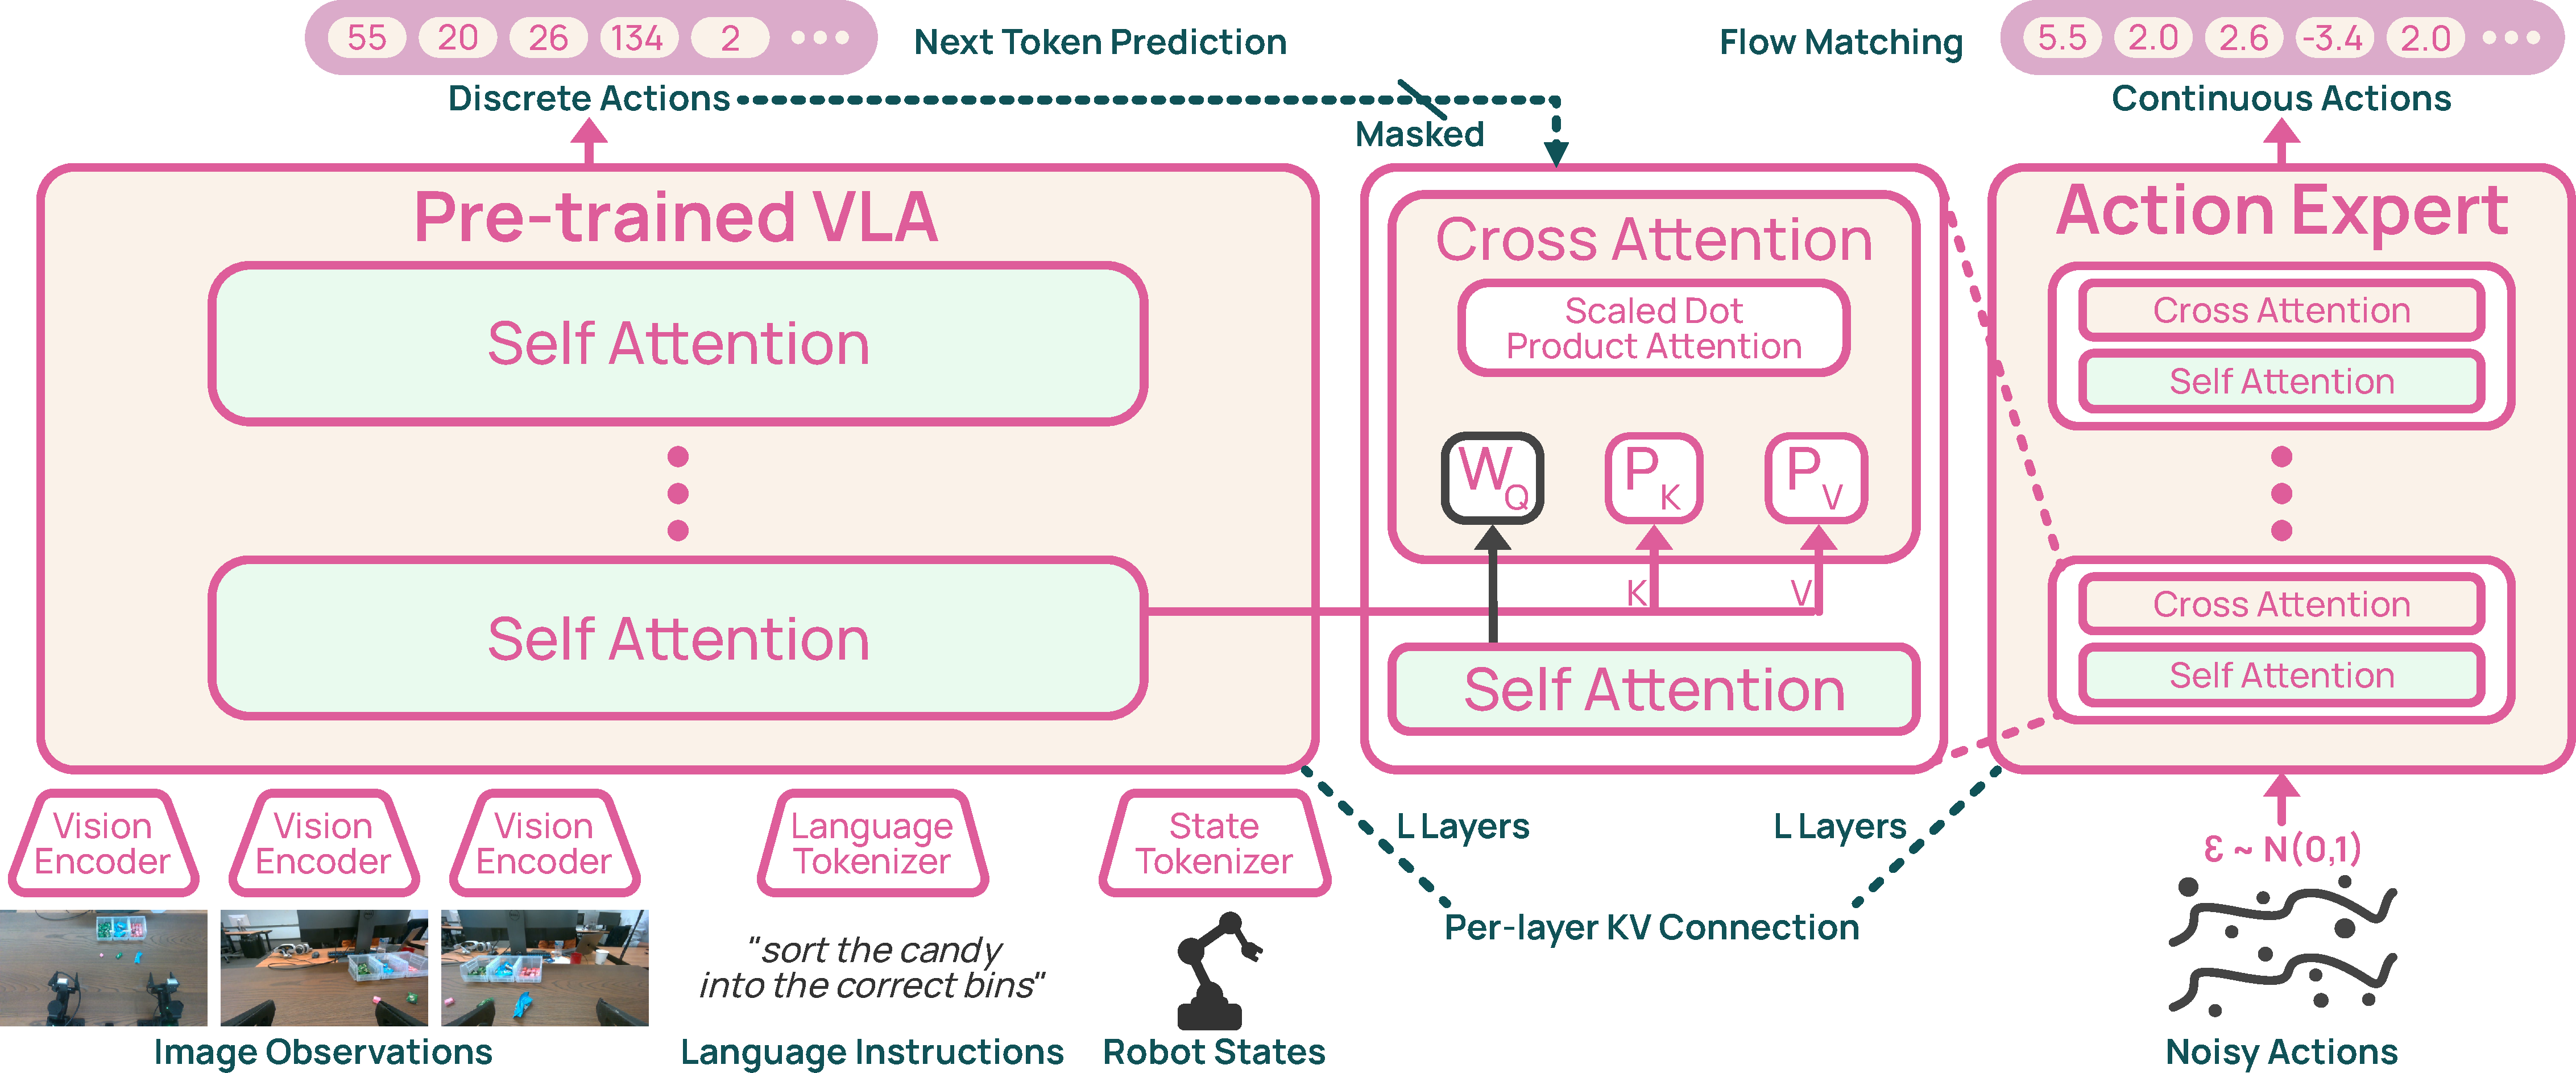
\includegraphics[width=\linewidth]{figures/MAF3.pdf}
\caption{\textbf{Overview of \molmoactt.} Image observations, language
instructions, and robot states are tokenized and processed by a pre-trained
VLA backbone with self-attention layers. Post-training attaches a DiT-style
action expert with the same number of layers as the backbone. At each layer,
the backbone key and value tensors are projected and reused as the key and
value inputs to the action expert's cross-attention, enabling per-layer KV
conditioning from visual-language context to continuous control. The expert is
trained with flow matching to denoise a noisy action trajectory into a
continuous robot trajectory. During training, the backbone is also supervised
with next-token prediction over discrete action tokens, while the target
action-token span is masked from the expert so continuous action prediction
cannot condition on the ground-truth discrete actions.}
\label{fig:overview}
\end{figure}


\molmoacttpre learns a robot policy through the same autoregressive interface used by the VLM: given language, visual observations, setup/control descriptors, and state tokens, it predicts discrete action tokens produced by \molmoactfast. This makes large-scale robot pre-training simple and stable, but the deployed policy should output continuous action trajectories directly. Post-training therefore adds a flow-matching action expert to the pre-trained VLM, producing the final \molmoactt model.

This section describes the two parts of that adaptation. First, we introduce the action expert and its per-layer KV conditioning on the VLM, which lets the continuous controller condition on the full visual-language attention state without replacing the backbone. Second, we describe the post-training recipe: how we keep the pre-training data construction, co-train discrete and continuous action supervision, mask padded or target-leaking tokens, and adjust packing and sequence lengths for the added action-expert compute. Additional model hyperparameters and implementation details are given in \autoref{supp:model-action-expert}, with shared training-system details in \autoref{supp:training}.

\subsubsection{Action expert and per-layer KV conditioning}
\label{sec:posttraining-action-expert}

Post-training adds a continuous action expert on top of the pre-trained autoregressive VLM. We use a DiT-style transformer expert because flow matching and diffusion models have shown that denoising transformers scale well for continuous generation, and because action trajectories are naturally represented as short continuous sequences rather than as text-like token streams. This choice separates responsibilities: the VLM provides visual-language grounding and robot-state context, while the expert models the continuous velocity field needed to transform noisy action chunks into executable trajectories.

The key architectural question is how this expert should receive VLM context. A shallow projection of the final hidden state compresses the backbone into a single residual-stream representation. Instead, \molmoactt conditions the expert on the VLM at every layer. Each action-expert block cross-attends to the corresponding VLM layer's keys and values, after lightweight learned projections map the VLM attention state into the expert's cross-attention width. This gives the continuous controller access to the same attention state used by the VLM itself, while preserving a modular interface between the backbone computation and the newly trained action expert.

Given a normalized target action chunk \(a\), Gaussian noise \(\epsilon\), and a sampled time \(t \in [0,1]\), we interpolate between noise and data,
\begin{equation}
    x_t = (1-t)\epsilon + t a,
    \qquad
    u^\star = a - \epsilon.
\end{equation}
The expert \(f_\theta\) predicts the target velocity \(u^\star\) from the noisy action chunk, the time embedding, and the VLM context \(c\), which contains the task, visual observations, setup/control descriptors, and discrete state tokens:
\begin{equation}
    \mathcal{L}_{\mathrm{flow}}
    =
    \mathbb{E}_{a,\epsilon,t}
    \left[
    \left\|
    m \odot \left(f_\theta(x_t,t,c) - u^\star\right)
    \right\|_2^2
    \right],
\end{equation}
where \(m\) masks padded action steps and padded action dimensions. At inference, we start from Gaussian noise and integrate the predicted velocity field to produce a continuous action trajectory.

Architecturally, the expert has the same depth as the VLM, where both of them use \(L=36\) layers. The expert first embeds the current noisy action sequence. Each block then applies action self-attention, cross-attention to the VLM, and an MLP, with the time embedding producing DiT-style shift, scale, and gate parameters for all three residual branches. Schematically, block \(\ell\) computes
\begin{align}
    h'_\ell
        &= h_\ell + g^{\mathrm{sa}}_\ell
        \operatorname{SA}\!\left(\operatorname{AdaRMS}^{\mathrm{sa}}_\ell(h_\ell,t)\right), \\
    \bar{h}_\ell
        &= h'_\ell + g^{\mathrm{ca}}_\ell
        \operatorname{CA}\!\left(
            \operatorname{AdaRMS}^{\mathrm{ca}}_\ell(h'_\ell,t),
            \tilde{K}_\ell,
            \tilde{V}_\ell
        \right), \\
    h_{\ell+1}
        &= \bar{h}_\ell + g^{\mathrm{ff}}_\ell
        \operatorname{MLP}\!\left(\operatorname{AdaRMS}^{\mathrm{ff}}_\ell(\bar{h}_\ell,t)\right).
\end{align}

The action expert uses per-layer KV conditioning rather than hidden-state conditioning. For each VLM layer \(\ell\), we collect the keys and values \((K^{\mathrm{vlm}}_\ell,V^{\mathrm{vlm}}_\ell)\) produced by that layer's self-attention. We then project them into the action-expert width with learned adapter projections \(P_K\) and \(P_V\):
\begin{equation}
    \tilde{K}_\ell =
    \operatorname{reshape}\!\left(P_K K^{\mathrm{vlm}}_\ell\right),
    \qquad
    \tilde{V}_\ell =
    \operatorname{reshape}\!\left(P_V V^{\mathrm{vlm}}_\ell\right).
\end{equation}
Here, \(P_K\) and \(P_V\) are linear VLM-to-expert adapter layers that align the VLM KV dimensionality with the expert's cross-attention width; they are separate from the VLM self-attention projections that produced the keys and values. After projection, the conditioning context is organized into the expert's attention heads. The cross-attention in expert block \(\ell\) attends to the projected keys and values from the corresponding VLM layer:
\begin{equation}
    \operatorname{CA}(Q_\ell,\tilde{K}_\ell,\tilde{V}_\ell)
    =
    \operatorname{softmax}\!\left(
        \frac{Q_\ell \tilde{K}_\ell^\top}{\sqrt{d_h}}
    \right)\tilde{V}_\ell,
\end{equation}
where \(d_h\) is the expert head dimension. This per-layer KV conditioning gives every action-expert block direct access to the visual-language attention state at the same depth in the backbone. During post-training we detach this conditioning path from the VLM, so the flow loss trains the expert and its adapter projections without sending gradients back through the VLM keys and values.

\subsubsection{Post-training recipe}
\label{sec:posttraining-recipe}

\paragraph{Overview.}
Post-training starts from the 200K-step \molmoacttpre checkpoint and turns it into the final \molmoactt model. We keep the VLM architecture and pre-training data construction from Sec.~\ref{sec:pretraining-recipe}, including the image augmentation described in \autoref{supp:training}. The main change is that robot examples now supervise both output interfaces: the LLM continues to predict discrete action tokens, while the action expert described in Sec.~\ref{sec:posttraining-action-expert} learns to generate continuous action chunks.

\paragraph{Multiple flow samples.}
For each robot action chunk, we evaluate the flow objective at multiple noise levels. Let \(a\) be a normalized continuous action chunk and \(c\) be the VLM context for the corresponding robot prompt. For each training example we draw \(K\) independent pairs \(\{(\epsilon_i,t_i)\}_{i=1}^K\), form \(x_{t_i}=(1-t_i)\epsilon_i+t_i a\), and train the expert to predict \(a-\epsilon_i\):
\begin{equation}
    \mathcal{L}_{\mathrm{flow}}(a,c)
    =
    \frac{1}{K}
    \sum_{i=1}^{K}
    \left\|
    m \odot
    \left(
    f_\theta(x_{t_i},t_i,c) - (a-\epsilon_i)
    \right)
    \right\|_2^2 .
\end{equation}
We use \(K=4\), so each robot sample contributes four points on the same flow trajectory while reusing the same visual-language context. We didn't use \(K=8\) as in the fine-tuning stage (Sec.~\ref{sec:finetuning}) mainly due to GPU memory constraints.

\paragraph{Padding and packing.}
Post-training retains a common action tensor shape across embodiments. Continuous actions are right-padded to a maximum horizon of 30 steps and a maximum width of 32 dimensions. The horizon mask removes padded time steps from the flow loss, and the dimension mask zeroes padded action dimensions in the noisy inputs, targets, and predictions before averaging the loss over valid dimensions. This lets datasets with different control rates and action widths share the same expert without training on artificial padded coordinates.

Packing is also extended to the continuous expert. A packed language sequence can contain multiple robot examples; each action chunk is paired with the sub-example that produced it, and the expert attends only to that example's VLM context. To keep memory use stable when packed batches contain different numbers of robot chunks, we pad the packed action-chunk axis up to a small fixed cap of five chunks per packed sequence when possible. Padded chunk rows are marked invalid and excluded from the flow loss; sequences with more chunks are still used, but processed without this fixed-cap padding.

\paragraph{Training objectives.}
The post-training objective combines the autoregressive loss from pre-training with the flow-matching loss:
\begin{equation}
    \mathcal{L}_{\mathrm{post}}
    =
    \mathcal{L}_{\mathrm{LM}}
    +
    \mathcal{L}_{\mathrm{flow}} .
\end{equation}
The language-model loss is applied to the same next-token targets used in pre-training, including discrete action tokens for robot examples and text tokens for VLM examples. The flow loss is applied only to continuous robot action chunks. Since robot examples contain both the discrete action target and the continuous action target, we mask the discrete action-token span out of the expert's VLM conditioning path. The expert therefore conditions on the task, observations, setup/control descriptors, and state tokens, but not on the target action tokens it is supposed to predict.

We also apply knowledge insulation \citep{driess2025knowledgeinsulation}, where the VLM is isolated from the continuous-action loss. The expert conditions on the VLM keys and values, but these tensors are detached before they enter the expert, so \(\mathcal{L}_{\mathrm{flow}}\) updates the action expert and its adapter projections without back-propagating through the VLM. The VLM is still updated by \(\mathcal{L}_{\mathrm{LM}}\).

\paragraph{Training.}
Robot batches use a sequence length of 2100 tokens, while the non-robot VLM batches keep the 4200-token context length from pre-training. We use this split because robot batches additionally run the action expert and four flow samples per action chunk, whereas VLM batches only train the autoregressive model. We train for 100K updates with a global batch size of 128 and a device batch size of 2 across 64 H100 GPUs for around 2,304 GPU hours. The VLM learning rates match pre-training: \(5\times10^{-6}\) for the vision encoder and connector, and \(1\times10^{-5}\) for the language model. The action expert is trained with a larger learning rate of \(5\times10^{-5}\).
